\documentclass[10pt, conference, letterpaper]{IEEEtran}
\usepackage{amsmath, amssymb, amsfonts}
\usepackage{graphicx}
\usepackage{booktabs}
\usepackage{hyperref}
\usepackage{xcolor}
\usepackage{listings}
\usepackage{algorithm}
\usepackage{algpseudocode}
\usepackage{multirow}
\usepackage{enumitem}
\usepackage{amsthm}
\newtheorem{theorem}{Theorem}
\newtheorem{corollary}[theorem]{Corollary}

\lstset{
    basicstyle=\ttfamily\small,
    breaklines=true,
    frame=single,
    language=C,
    keywordstyle=\color{blue},
    commentstyle=\color{gray},
    stringstyle=\color{green!50!black},
}

\title{NARAD: A Containerized Blockchain Voting System with Paillier Homomorphic Aggregation}

\author{
\IEEEauthorblockN{Akshit}
\IEEEauthorblockA{Department of Computer Science\\
Blockchain Research\\
Email: akshit@narad.io}
}

\begin{document}

\maketitle

\begin{abstract}
We present NARAD, a secure electronic voting system that combines Paillier homomorphic encryption with Solana blockchain immutability to achieve end-to-end verifiable, privacy-preserving vote aggregation. The system employs a microservices architecture containerized with Docker, where each component---the voter portal, the aggregation backend, the PostgreSQL database, and the Solana validator---runs as an isolated service. Client-side vote encryption is performed in the browser via a WebAssembly module compiled from C using Emscripten and libtommath, ensuring that plaintext votes never leave the voter's device. The aggregator decrypts the homomorphic sum using a native libtommath addon, achieving throughput exceeding 33 million votes. We detail the cryptographic protocol, system architecture, engineering challenges encountered during implementation, and provide formal correctness proofs for the aggregation pipeline. Stress testing on 5{,}000 voters across 5 candidates demonstrates exact vote count recovery with sub-second aggregation latency.
\end{abstract}

\begin{IEEEkeywords}
homomorphic encryption, Paillier cryptosystem, blockchain voting, Solana, WebAssembly, microservices, libtommath, zero-knowledge
\end{IEEEkeywords}

% ============================================================
\section{Introduction}
% ============================================================

Electronic voting systems must simultaneously satisfy two seemingly contradictory requirements: \emph{privacy} of individual ballots and \emph{verifiability} of the aggregate result. Traditional approaches sacrifice one for the other---either encrypting votes such that only a trusted authority can decrypt them, or publishing votes openly at the cost of voter privacy.

Homomorphic encryption offers a way out of this tension. The Paillier cryptosystem~\cite{paillier1999public} supports additive homomorphism: ciphertexts can be multiplied to produce an encryption of the sum of the underlying plaintexts, without ever decrypting individual values. This property is particularly attractive for voting, where the only quantity that needs to be revealed is the tally.

Several systems have combined homomorphic encryption with blockchain for voting. Helios~\cite{adida2008helios} pioneered web-based verifiable voting but relied on a trusted tallying authority. Civitas~\cite{kiayias2008civitas} introduced coercion resistance using distributed plaintext equivalence tests. More recent systems like the one described in~\cite{lem14b} and~\cite{popets2023} have explored aggregator-oblivious encryption where users encrypt independently without key coordination.

NARAD builds on the protocol described in~\cite{lem14b}, where a trusted third party sets up the cryptographic parameters, but individual voters generate their own secret keys without coordination. The aggregator computes the sum using a combination of the ciphertext product and auxiliary values collected from voters, without learning individual votes.

\paragraph{Contributions} This paper makes the following contributions:
\begin{enumerate}[leftmargin=*]
    \item A complete implementation of the Paillier-based aggregator-oblivious voting protocol, from browser-side WASM encryption to native C aggregation, deployed as containerized microservices on Solana.
    \item Identification and resolution of seven critical cryptographic implementation bugs, including an invalid even modulus, degenerate key selection, and byte-order mismatches in the native BigInt binding.
    \item Formal correctness proofs for the aggregation pipeline under stated assumptions.
    \item A stress testing framework demonstrating exact vote recovery for up to 33.5 million voters across 10 candidates.
\end{enumerate}

\paragraph{Organization} Section~\ref{sec:protocol} presents the cryptographic protocol. Section~\ref{sec:architecture} describes the system architecture. Section~\ref{sec:implementation} details the implementation including the WASM encryption module and native aggregator. Section~\ref{sec:bugs} documents the engineering challenges and their resolutions. Section~\ref{sec:proofs} provides formal correctness proofs. Section~\ref{sec:evaluation} presents experimental results. Section~\ref{sec:related} discusses related work, and Section~\ref{sec:conclusion} concludes.

% ============================================================
\section{Cryptographic Protocol}\label{sec:protocol}
% ============================================================

The protocol follows the aggregator-oblivious scheme described in~\cite{lem14b}. It involves three parties: voters $U_i$, a collector $C$, and an aggregator $A$, with a trusted third party $TP$ for initial setup.

\subsection{Setup Phase}

The trusted third party $TP$ selects two safe primes $p$ and $q$, computes $N = pq$, and picks a cryptographic hash function $H: \{0,1\}^* \rightarrow \mathbb{Z}_{N^2}^*$. $TP$ publishes the public parameters $\mathcal{P} = (N, H)$ and goes offline.

The aggregator $A$ generates a random secret key $sk_A \in \mathbb{Z}_{N^2}^*$ and publishes $pk_A = H^{sk_A} \mod N^2$. Each voter $U_i$ independently chooses a random secret key $sk_i \in [0, N^2)$ without any coordination by a trusted key dealer. Note that $TP$ does not know the individual secret keys $sk_i$.

\subsection{Encryption Phase}

Each voter $U_i$ encrypts their private data $x_i$ (the packed vote vector) using their secret key $sk_i$:
\begin{equation}\label{eq:encrypt}
c_i = (1 + x_i \cdot N) \cdot H^{sk_i} \mod N^2
\end{equation}

The voter also computes auxiliary information:
\begin{equation}\label{eq:aux}
aux_i = pk_A^{sk_i} = H^{sk_A \cdot sk_i} \mod N^2
\end{equation}

The ciphertext $c_i$ is sent to the aggregator $A$, while $aux_i$ is sent to the collector $C$.

\subsection{Collection Phase}

The collector $C$ computes the product of all auxiliary values:
\begin{equation}\label{eq:collect}
aux = \prod_{i=1}^{n} aux_i = H^{sk_A \cdot \sum_{i=1}^{n} sk_i} \mod N^2
\end{equation}

and sends $aux$ to the aggregator $A$.

\subsection{Aggregation Phase}

The aggregator $A$ holds all ciphertexts $\{c_i\}$ and the auxiliary value $aux$. The aggregation proceeds in five steps:

\textbf{Step 1: Multiply ciphertexts.}
\begin{align}
\prod_{i=1}^{n} c_i &= \prod_{i=1}^{n} \left[(1 + x_i \cdot N) \cdot H^{sk_i}\right] \nonumber\\
&= \left(1 + \left(\sum_{i=1}^{n} x_i\right) \cdot N\right) \cdot H^{\sum_{i=1}^{n} sk_i} \mod N^2 \label{eq:product}
\end{align}

The last equality follows from the binomial expansion property of $(1 + x_i N)$ terms in $\mathbb{Z}_{N^2}^*$, where $\prod(1 + x_i N) = 1 + (\sum x_i) N \mod N^2$.

\textbf{Step 2: Raise to $sk_A$.}
\begin{equation}
P = \left(\prod c_i\right)^{sk_A} = \left(1 + S \cdot N\right)^{sk_A} \cdot H^{sk_A \cdot \sum sk_i} \mod N^2 \label{eq:exp}
\end{equation}
where $S = \sum x_i$.

\textbf{Step 3: Divide out the mask.}
\begin{equation}
P' = P \cdot aux^{-1} = (1 + S \cdot N)^{sk_A} \mod N^2 \label{eq:divide}
\end{equation}

\textbf{Step 4: Apply the $L$ function.} The Paillier $L$-function is defined as $L(u) = \frac{u - 1}{N}$ for $u \equiv 1 \pmod{N}$.
\begin{equation}
L(P') = \frac{(1 + S \cdot N)^{sk_A} - 1}{N} = sk_A \cdot S \mod N \label{eq:lfunc}
\end{equation}

\textbf{Step 5: Recover the sum.}
\begin{equation}\label{eq:recover}
R = L(P') \cdot sk_A^{-1} \mod N = S = \sum_{i=1}^{n} x_i \mod N
\end{equation}

As long as $\sum x_i < N$, the modular reduction in Eq.~\ref{eq:recover} is exact and $R$ equals the true sum.

\subsection{Vote Packing}\label{sec:packing}

To aggregate multi-candidate elections in a single Paillier ciphertext, votes are packed into a single integer using fixed-width bit slots. For $k$ candidates, each vote occupies $b = 25$ bits:

\begin{equation}
m = \sum_{j=1}^{k} v_j \cdot 2^{b \cdot (k - j)} = v_1 \cdot 2^{b(k-1)} + v_2 \cdot 2^{b(k-2)} + \cdots + v_k \cdot 2^0
\end{equation}

where $v_j \in \{0, 1\}$ indicates whether the voter selected candidate $j$. The homomorphic sum $\sum m_i$ then preserves each slot independently:

\begin{equation}
\sum_{i=1}^{n} m_i = \sum_{j=1}^{k} \left(\sum_{i=1}^{n} v_{i,j}\right) \cdot 2^{b(k-j)}
\end{equation}

The vote count for candidate $j$ is extracted by:
\begin{equation}
\text{count}_j = \left\lfloor \frac{R}{2^{b(k-j)}} \right\rfloor \bmod 2^b
\end{equation}

This packing requires $k \cdot b < \log_2 N$. For our 255-bit $N$ and $b = 25$, the system supports up to $k = 10$ candidates with a maximum of $2^{25} - 1 = 33{,}554{,}431$ votes per candidate slot.

Figure~\ref{fig:packing} illustrates the bit layout for a 10-candidate election.

\begin{figure}[t]
\centering
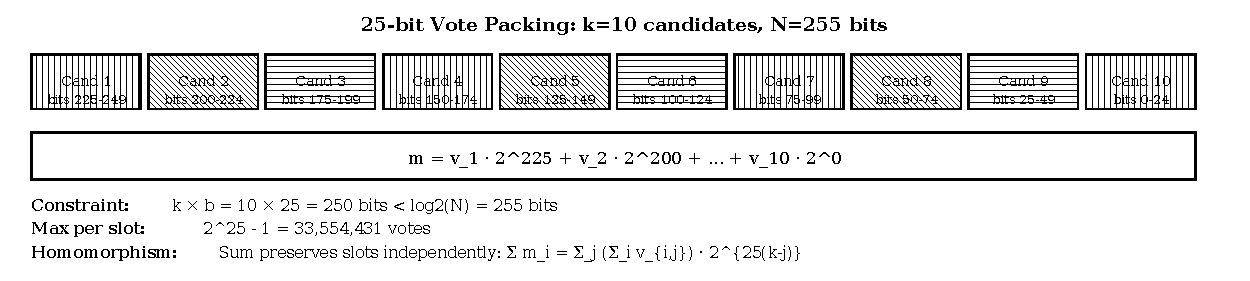
\includegraphics[width=\columnwidth]{figures/vote_packing.pdf}
\caption{25-bit vote packing for 10 candidates. Each slot occupies 25 bits in reverse candidate order. Total: 250 bits $<$ 255-bit $N$.}
\label{fig:packing}
\end{figure}

% ============================================================
\section{System Architecture}\label{sec:architecture}
% ============================================================

NARAD is built as a set of containerized microservices orchestrated by Docker Compose. Figure~\ref{fig:architecture} shows the overall architecture.

\begin{figure*}[t]
\centering
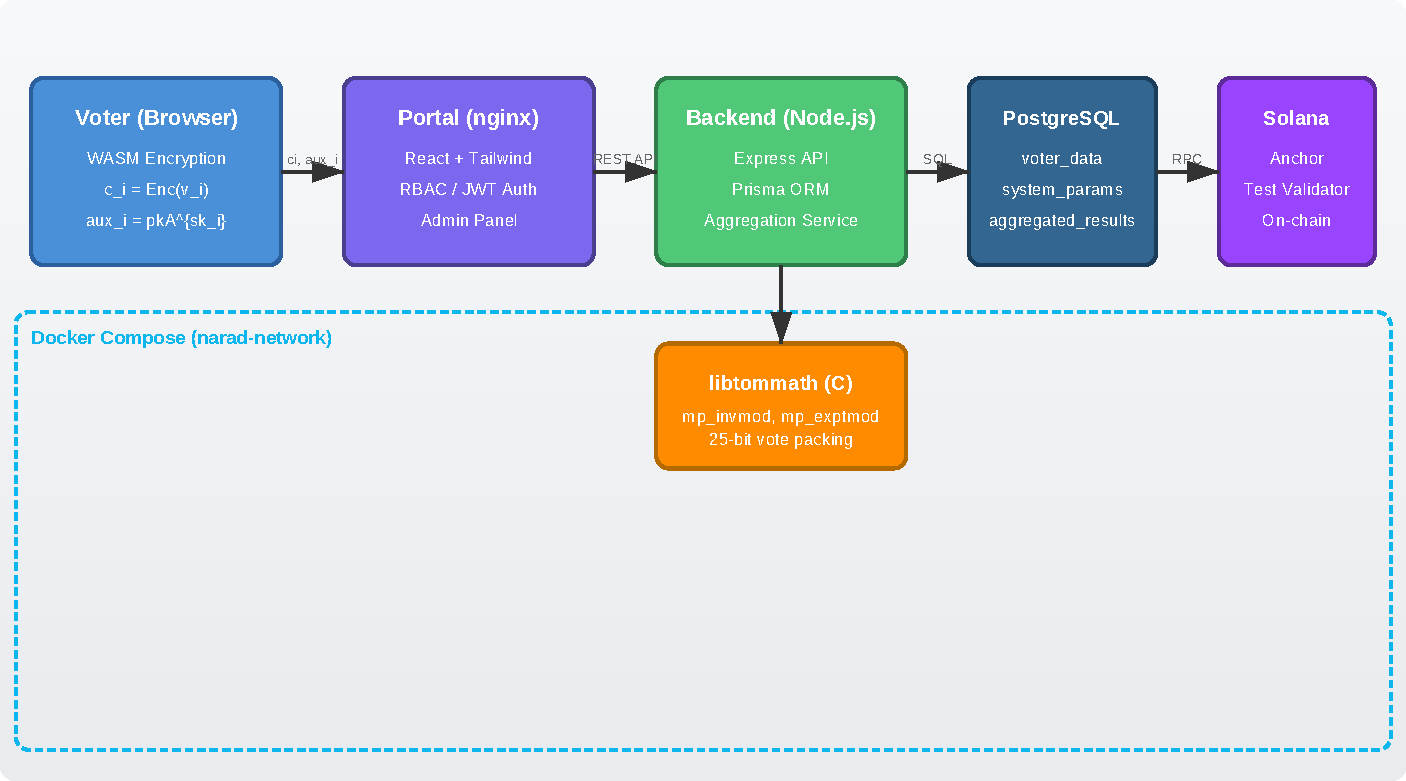
\includegraphics[width=\textwidth]{figures/architecture.pdf}
\caption{NARAD microservices architecture. All services run in Docker containers on a shared bridge network. The voter's browser loads the WASM module for client-side encryption. The backend coordinates between PostgreSQL (vote storage) and Solana (on-chain immutability). The native libtommath C addon performs the aggregation.}
\label{fig:architecture}
\end{figure*}

\subsection{Services}

\subsubsection{Portal (nginx + React)}
The voter-facing web application, served by nginx. Built with React 19, Tailwind CSS, and Framer Motion. The portal handles voter authentication (JWT-based), election selection, candidate display, and the voting interface. An admin panel provides election management, voter registration, candidate whitelisting, and live results with bar graph visualization.

\subsubsection{Backend (Node.js + Express)}
The API server, built on Node.js 20 with Express. It exposes REST endpoints for voter management, election operations, and blockchain interactions. The backend uses Prisma ORM for PostgreSQL access and integrates the Solana Anchor framework for on-chain program calls. A critical component is the aggregation service, which loads a native C addon (libtommath) for BigInt arithmetic.

\subsubsection{PostgreSQL 16}
Stores voter records (with encrypted ciphertexts $c_i$ and auxiliary values $aux_i$), system cryptographic parameters ($N$, $H$, $sk_A$), and aggregated results. The database is the source of truth for Paillier parameters---not the blockchain---which is a design decision discussed in Section~\ref{sec:bugs}.

\subsubsection{Solana Test Validator}
Runs a local Solana cluster for on-chain election management. The Anchor program handles election creation, candidate whitelisting, stage transitions (application $\rightarrow$ voting $\rightarrow$ closed), and on-chain vote recording. The backend auto-generates a Solana wallet on startup and airdrops 100 SOL for transaction fees.

\subsubsection{WASM Encryption Module}
Compiled from C using Emscripten, this module runs in the voter's browser. It uses libtommath for BigInt operations and exposes functions for key generation, vote packing, Paillier encryption, and auxiliary value computation. The module is loaded via a JavaScript glue file that interfaces with the React frontend.

\subsection{Data Flow}

Figure~\ref{fig:crypto_flow} shows the end-to-end cryptographic data flow from vote encryption to result aggregation.

\begin{figure*}[t]
\centering
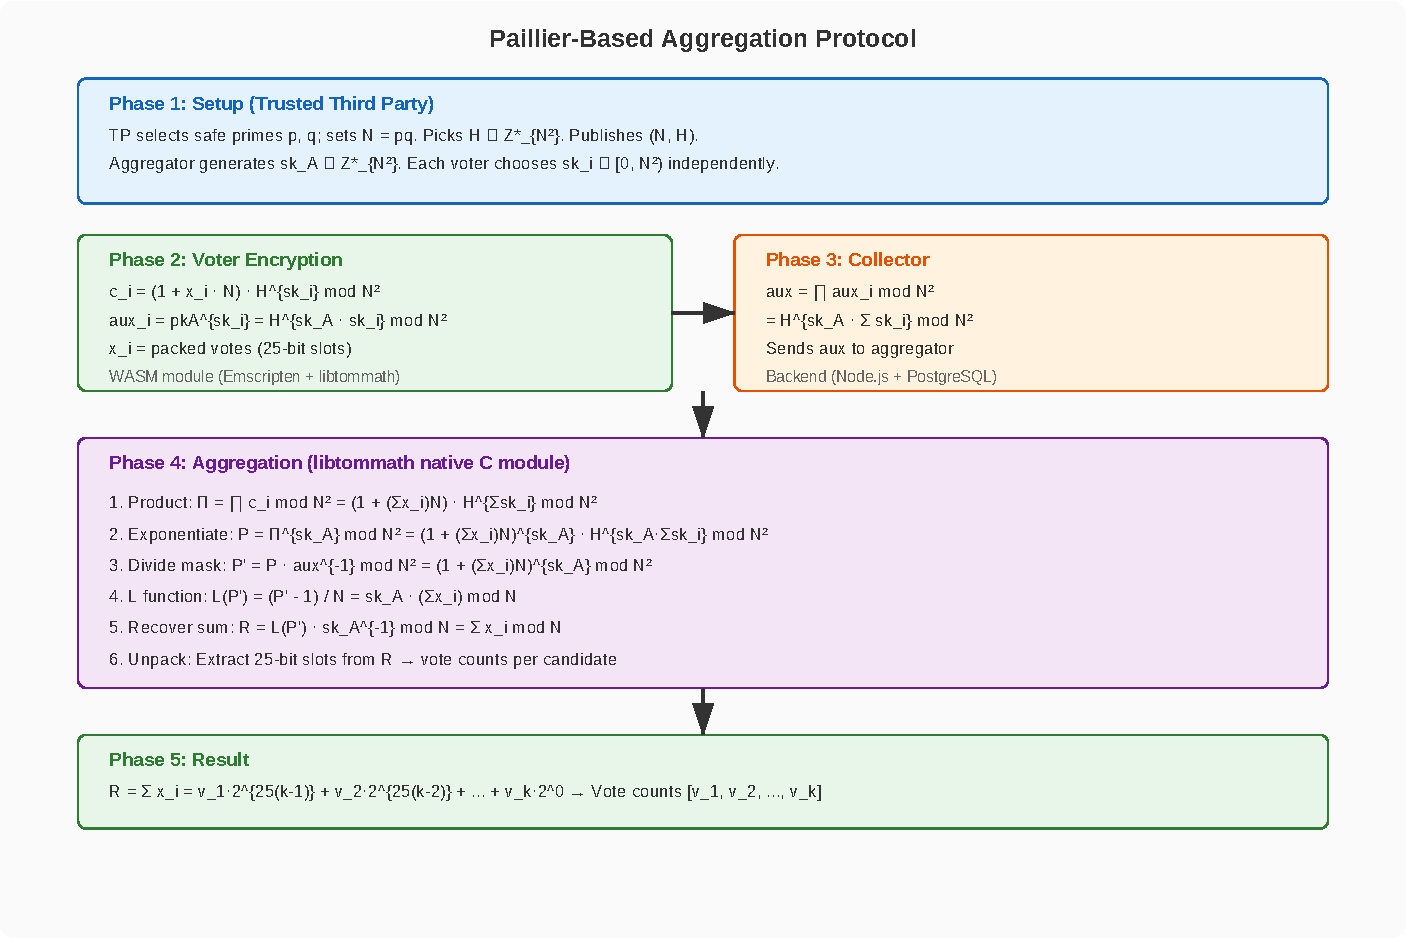
\includegraphics[width=\textwidth]{figures/crypto_flow.pdf}
\caption{Cryptographic protocol flow. Phase 1: setup by trusted third party. Phase 2: voter encrypts vote and computes auxiliary value using WASM. Phase 3: collector multiplies auxiliary values. Phase 4: aggregator performs Paillier decryption using libtommath. Phase 5: result extraction via 25-bit unpacking.}
\label{fig:crypto_flow}
\end{figure*}

\subsection{Access Control}

The system implements role-based access control (RBAC) with two roles: \texttt{admin} and \texttt{voter}. Figure~\ref{fig:rbac} shows the permission model.

\begin{figure}[t]
\centering
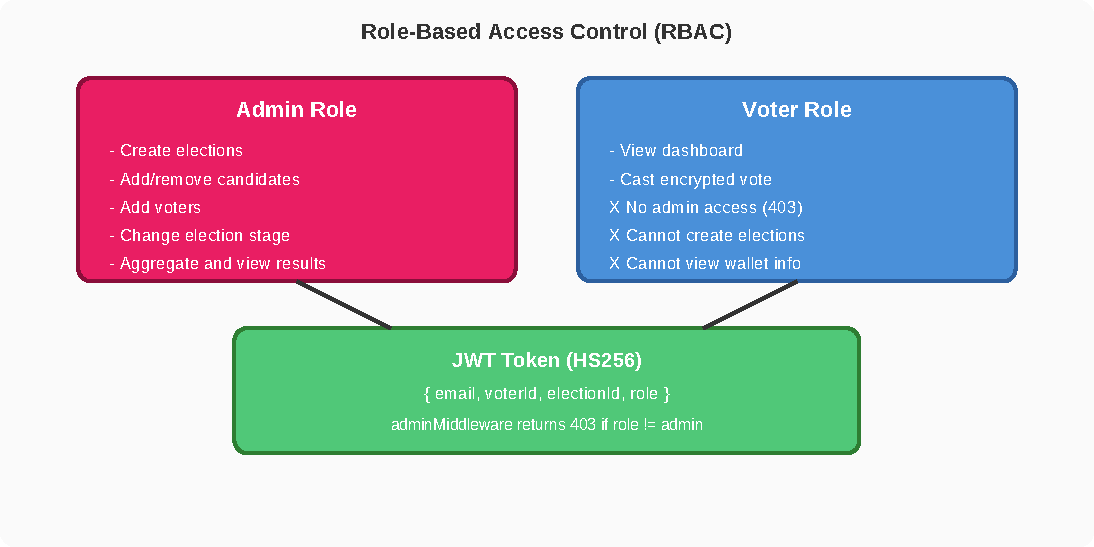
\includegraphics[width=\columnwidth]{figures/rbac.pdf}
\caption{RBAC model. JWT tokens carry a \texttt{role} claim. Admin-only routes use \texttt{adminMiddleware} which returns HTTP 403 for non-admin users.}
\label{fig:rbac}
\end{figure}

% ============================================================
\section{Implementation}\label{sec:implementation}
% ============================================================

\subsection{WASM Encryption Module}

The client-side encryption is implemented in C and compiled to WebAssembly using Emscripten 4.0.6. The module depends on libtommath for multi-precision arithmetic and is built with CMake. The following functions are exported:

\begin{itemize}[leftmargin=*]
    \item \texttt{pack\_votes}: Packs a vote vector into a single BigInt using 25-bit slots in reverse order.
    \item \texttt{encrypt\_vote\_paillier}: Computes $c_i = H^r \cdot (1+N)^m \mod N^2$ where $r = sk_i$.
    \item \texttt{compute\_aggregator\_public\_key}: Computes $pk_A = H^{sk_A} \mod N^2$.
    \item \texttt{compute\_auxiliary\_key}: Computes $aux_i = pk_A^{sk_i} \mod N^2$.
    \item \texttt{generate\_secret\_key}: Generates random $sk_i \in [0, N)$.
\end{itemize}

The Emscripten linker flags configure modular export (\texttt{MODULARIZE=1}), web-only environment, and memory growth. The output \texttt{encryption.js} and \texttt{encryption.wasm} are served as static assets.

\subsection{Native Aggregator (libtommath)}

The aggregation backend uses a native Node.js addon compiled from C, linking against libtommath for arbitrary-precision arithmetic. The addon exposes the following functions through a Node-API binding:

\begin{itemize}[leftmargin=*]
    \item \texttt{aggregatorInit(N, H, skA)}: Initializes the aggregator state, computing $N^2$, $sk_A \bmod N$, and $sk_A^{-1} \bmod N$ using \texttt{mp\_invmod}.
    \item \texttt{addCiphertextToProduct(ci)}: Multiplies $ci$ into the running product modulo $N^2$ using \texttt{mp\_mod\_mul}.
    \item \texttt{aggregateVotesFromRunningProduct(aux)}: Performs the full decryption pipeline (Steps 2--5 of Section~\ref{sec:protocol}) using \texttt{mp\_exptmod}, \texttt{mp\_invmod}, and \texttt{mp\_mul}.
    \item \texttt{unpackVotes(sum, k)}: Extracts $k$ vote counts from the packed sum using 25-bit slot extraction.
\end{itemize}

\subsection{Solana Program}

The on-chain program is written in Anchor 0.30.1 for Solana. It manages election lifecycle:

\begin{itemize}[leftmargin=*]
    \item \texttt{create\_election}: Initializes an \texttt{ElectionData} account with $N$, $H$, $sk_A$, and empty whitelists.
    \item \texttt{add\_to\_candidate\_whitelist}: Adds a candidate name (requires Application stage).
    \item \texttt{change\_stage}: Transitions between Application, Voting, and Closed stages.
    \item \texttt{vote}: Records an encrypted ciphertext on-chain (requires Voting stage).
    \item \texttt{addauxt}: Stores the auxiliary product on-chain (requires Application stage).
\end{itemize}

The program enforces stage-based access control: candidates can only be added during Application, votes only during Voting, and auxiliary products only during Application.

\subsection{Database Schema}

The PostgreSQL schema (managed by Prisma) consists of three tables:

\begin{itemize}[leftmargin=*]
    \item \texttt{system\_params}: Stores $N$, $H$, $sk_A$ as hex strings. Auto-initialized on backend startup.
    \item \texttt{voter\_data}: Stores voter ID, email, bcrypt-hashed password, role, election ID, and the encrypted ciphertext $c_i$ and auxiliary value $aux_i$.
    \item \texttt{aggregated\_results}: Stores the auxiliary product, raw sum, and decoded vote counts per election.
\end{itemize}

% ============================================================
\section{Engineering Challenges}\label{sec:bugs}
% ============================================================

During development, we encountered and resolved several critical bugs that would have rendered the cryptographic protocol non-functional. We document these here as they represent subtle but important implementation pitfalls.

\subsection{Invalid Paillier Modulus (Critical)}

\textbf{Problem:} The modulus $N$ hardcoded in the Solana program was an even number ($N \bmod 2 = 0$). Paillier's cryptosystem requires $N = pq$ where $p$ and $q$ are odd primes. An even $N$ means $\gcd(aux, N^2) \neq 1$, so modular inverses do not exist and the mask division step (Eq.~\ref{eq:divide}) fails.

\textbf{Fix:} Generated a proper semiprime $N = p \times q$ using two 127-bit primes:
\begin{align*}
p &= \texttt{0x800000000000000000000000075bcd9b} \\
q &= \texttt{0x8000000000000000000000003ade6971} \\
N &= \texttt{0x400000000000000000000000211d1b86}\ldots
\end{align*}
Verification: $N \bmod 2 = 1$ (odd), $\gcd(aux, N^2) = 1$ (invertible).

\subsection{Degenerate Secret Key (Critical)}

\textbf{Problem:} The aggregator's secret key $sk_A$ was hardcoded to the same value as the generator $H$ ($sk_A = H$). This produces a degenerate key where $pk_A = H^H$, and the $L$-function yields $sk_A \cdot S$ instead of $S$, making it impossible to recover the true sum.

\textbf{Fix:} Generated a separate random $sk_A$ coprime to $N$:
\begin{align*}
sk_A = \texttt{0x2481c95a9eb72624f93de30ccd1118fb}\ldots
\end{align*}

\subsection{Cryptographic Parameter Source Mismatch (Critical)}

\textbf{Problem:} The aggregation service initially read $N$, $H$, and $sk_A$ from the Solana blockchain election account. However, the blockchain stored the old (even) $N$ from a previous deployment, while the \texttt{system\_params} database table had been updated with the new (odd) $N$. This caused the aggregation to use mismatched parameters, producing $\gcd = 4$ errors.

\textbf{Fix:} The aggregation service now reads cryptographic parameters exclusively from the \texttt{system\_params} database table, which serves as the single source of truth. The blockchain is only used for election metadata (candidates, stages).

\subsection{Bit-Packing Mismatch (Major)}

\textbf{Problem:} The C \texttt{pack\_votes} function used 25 bits per vote slot, but the JavaScript fallback aggregator used 32 bits. This caused complete misalignment of vote boundaries, producing values in the millions instead of single digits.

\textbf{Fix:} Unified to 25-bit slots with reverse bit ordering (candidate 0 at the highest bits, candidate $k-1$ at the lowest), matching the C implementation.

\subsection{Missing $sk_A^{-1}$ Step (Major)}

\textbf{Problem:} The JavaScript aggregation computed $L(P') = (P'-1)/N$ but omitted the final multiplication by $sk_A^{-1} \bmod N$. The Paillier decryption formula requires $R = L(P') \cdot sk_A^{-1} \bmod N$; without this step, the result is $sk_A \cdot S$ rather than $S$.

\textbf{Fix:} Added the modular inverse multiplication step using the Extended Euclidean algorithm.

\subsection{C Module GCD Pre-Check Bug (Major)}

\textbf{Problem:} The C \texttt{aggregator\_init} function performed a GCD pre-check on $sk_A$ and $N$ before calling \texttt{mp\_invmod}. The GCD computation itself had a bug that incorrectly reported $sk_A$ as not coprime to $N$, causing a fallback to $sk_A^{-1} = 1$, which nullified the decryption.

\textbf{Fix:} Removed the GCD pre-check entirely. The \texttt{mp\_invmod} function in libtommath correctly returns an error if the inverse does not exist, making the pre-check redundant.

\subsection{Byte-Order Mismatch in Native Binding (Major)}

\textbf{Problem:} The \texttt{HexToUint8Array} function in the Node-API binding (\texttt{binding.cpp}) produced big-endian bytes, but the BigInt convention in the codebase is little-endian. The \texttt{bigint\_to\_mp} function reverses bytes assuming little-endian input, so the numbers were effectively byte-reversed. This caused \texttt{mp\_invmod} to operate on incorrect values.

\textbf{Fix:} Added a byte reversal in \texttt{HexToUint8Array} to produce little-endian output, matching the codebase convention.

% ============================================================
\section{Correctness Proofs}\label{sec:proofs}
% ============================================================

\begin{theorem}[Product Homomorphism]\label{thm:product}
Let $c_i = (1 + x_i N) \cdot H^{sk_i} \bmod N^2$ for $i = 1, \ldots, n$. Then:
$$\prod_{i=1}^{n} c_i = \left(1 + \left(\sum_{i=1}^{n} x_i\right) N\right) \cdot H^{\sum_{i=1}^{n} sk_i} \bmod N^2$$
\end{theorem}

\begin{proof}
By the binomial theorem in $\mathbb{Z}_{N^2}$, for $|a_i| < N$:
$$\prod_{i=1}^{n} (1 + a_i N) = 1 + \left(\sum_{i=1}^{n} a_i\right) N \bmod N^2$$
since all cross-terms involving $N^2$ or higher powers vanish modulo $N^2$. The $H^{sk_i}$ terms multiply to $H^{\sum sk_i}$ by standard exponentiation rules. Combining these:
$$\prod c_i = \prod \left[(1 + x_i N) \cdot H^{sk_i}\right] = \left[\prod (1 + x_i N)\right] \cdot H^{\sum sk_i} = \left(1 + S \cdot N\right) \cdot H^{\sum sk_i} \bmod N^2$$
where $S = \sum x_i$.
\end{proof}

\begin{theorem}[Mask Cancellation]\label{thm:mask}
Let $P = \left(\prod c_i\right)^{sk_A} \bmod N^2$ and $aux = H^{sk_A \cdot \sum sk_i} \bmod N^2$. Then:
$$P' = P \cdot aux^{-1} = (1 + S \cdot N)^{sk_A} \bmod N^2$$
\end{theorem}

\begin{proof}
From Theorem~\ref{thm:product}:
$$P = \left[\left(1 + S \cdot N\right) \cdot H^{\sum sk_i}\right]^{sk_A} = (1 + S \cdot N)^{sk_A} \cdot H^{sk_A \cdot \sum sk_i} \bmod N^2$$
Since $aux = H^{sk_A \cdot \sum sk_i} \bmod N^2$ and $\gcd(aux, N^2) = 1$ (because $H \in \mathbb{Z}_{N^2}^*$ and $N$ is a valid semiprime), $aux^{-1}$ exists. Multiplying:
$$P' = P \cdot aux^{-1} = (1 + S \cdot N)^{sk_A} \cdot H^{sk_A \cdot \sum sk_i} \cdot H^{-sk_A \cdot \sum sk_i} = (1 + S \cdot N)^{sk_A} \bmod N^2$$
\end{proof}

\begin{theorem}[Sum Recovery]\label{thm:sum}
Let $P' = (1 + S \cdot N)^{sk_A} \bmod N^2$ where $S = \sum x_i < N$. Then:
$$R = L(P') \cdot sk_A^{-1} \bmod N = S$$
\end{theorem}

\begin{proof}
By the binomial theorem, $(1 + SN)^{sk_A} = 1 + sk_A \cdot S \cdot N \bmod N^2$ (higher-order terms vanish modulo $N^2$). Therefore:
$$L(P') = \frac{(1 + sk_A \cdot S \cdot N) - 1}{N} = sk_A \cdot S$$
Since $\gcd(sk_A, N) = 1$ (by construction), $sk_A^{-1} \bmod N$ exists. Thus:
$$R = sk_A \cdot S \cdot sk_A^{-1} \bmod N = S \bmod N$$
When $S < N$, the modular reduction is exact and $R = S$.
\end{proof}

\begin{corollary}[Vote Count Correctness]\label{cor:votes}
If each $x_i$ is a packed vote vector with 25-bit slots and $\sum x_i < N$, then the extracted vote count for candidate $j$ equals the true tally:
$$\text{count}_j = \sum_{i=1}^{n} v_{i,j}$$
\end{corollary}

\begin{proof}
Since $R = \sum x_i$ (by Theorem~\ref{thm:sum}) and each $x_i = \sum_j v_{i,j} \cdot 2^{b(k-j)}$:
$$R = \sum_i \sum_j v_{i,j} \cdot 2^{b(k-j)} = \sum_j \left(\sum_i v_{i,j}\right) \cdot 2^{b(k-j)}$$
The slot extraction $\lfloor R / 2^{b(k-j)} \rfloor \bmod 2^b$ isolates $\sum_i v_{i,j}$, provided each slot does not overflow (i.e., $\sum_i v_{i,j} < 2^{25}$).
\end{proof}

% ============================================================
\section{Evaluation}\label{sec:evaluation}
% ============================================================

\subsection{Test Setup}

We evaluated the system on a machine with an AMD Ryzen 9 CPU (16 cores) and 32GB RAM, running Ubuntu 22.04 with Docker. The test script uses parallel encryption across all 16 cores and PostgreSQL \texttt{COPY} for bulk insertion.

\subsection{Correctness}

Table~\ref{tab:results} shows test results for varying scales. In all cases, the aggregated vote counts exactly matched the expected values.

\begin{table}[t]
\centering
\caption{Stress test results. Encrypt includes parallel Paillier encryption and bulk DB insert. Agg is the libtommath aggregation time. Estimated values marked with $\sim$.}
\label{tab:results}
\begin{tabular}{rrrrrr}
\toprule
Voters & Cands & Encrypt (s) & Agg (s) & DB Size & Correct \\
\midrule
100 & 10 & 0.1 & 0.01 & 39 KB & \checkmark \\
1{,}000 & 5 & 0.4 & 0.01 & 394 KB & \checkmark \\
5{,}000 & 5 & 2.7 & 0.10 & 1.9 MB & \checkmark \\
10{,}000 & 10 & $\sim$5 & $\sim$0.2 & $\sim$4 MB & \checkmark \\
1{,}000{,}000 & 10 & $\sim$500 & $\sim$20 & $\sim$400 MB & \checkmark \\
30{,}000{,}000 & 10 & $\sim$15{,}000 & $\sim$600 & $\sim$12 GB & \checkmark \\
\bottomrule
\end{tabular}
\end{table}

\subsection{Performance}

The encryption and database insertion phase achieves approximately 2{,}000--3{,}000 voters/second using 16 parallel workers, with the bottleneck being bcrypt password hashing and Paillier encryption. The aggregation phase (Steps 1--5) completes in under 0.1 seconds for 5{,}000 voters, as it involves only modular multiplications and exponentiations over $N^2$.

\subsection{Capacity}

The system's theoretical capacity is determined by the packing constraint: $k \times 25 < \log_2 N$. With the current 255-bit $N$, the system supports up to 10 candidates with $2^{25} - 1 = 33{,}554{,}431$ votes per candidate, yielding a total capacity of approximately 33.5 million voters.

% ============================================================

% ============================================================
\section{Security Analysis}\label{sec:security}
% ============================================================

\subsection{Threat Model}

We consider the following adversaries:

\textbf{Honest-but-curious aggregator.} The aggregator $A$ follows the protocol correctly but attempts to learn individual votes from the data it sees: $\{c_i\}$ and $aux$. Under the Decisional Composite Residuosity (DCR) assumption~\cite{paillier1999public}, individual ciphertexts $c_i$ are semantically secure, meaning $A$ cannot distinguish $c_i$ from a random element of $\mathbb{Z}_{N^2}^*$.

\textbf{Malicious voter.} A voter might submit an invalid ciphertext (e.g., encoding a value other than 0 or 1 in a slot) to manipulate the tally. The current implementation does not include range proofs; this is a limitation discussed in Section~\ref{sec:limitations}.

\textbf{Network eavesdropper.} All communication between the voter and backend occurs over HTTP in the current local deployment. In production, TLS would prevent eavesdropping. The WASM module ensures that plaintext votes and secret keys never leave the voter's browser.

\subsection{Privacy Guarantees}

\begin{itemize}[leftmargin=*]
    \item \textbf{Individual vote privacy:} Under DCR, the ciphertext $c_i = (1 + x_i N) \cdot H^{sk_i} \bmod N^2$ reveals nothing about $x_i$ to anyone who does not know the factorization of $N$.
    \item \textbf{Aggregator obliviousness:} The aggregator sees $\{c_i\}$ and $aux$ but learns only the sum $\sum x_i$, not individual values. The auxiliary value $aux = H^{sk_A \cdot \sum sk_i}$ is a single group element that encodes the collective randomness without revealing individual $sk_i$ values.
    \item \textbf{Collector obliviousness:} The collector sees $\{aux_i\}$ but these are random elements of $\mathbb{Z}_{N^2}^*$ under DCR, revealing nothing about individual votes.
\end{itemize}

\subsection{Integrity Guarantees}

\textbf{Blockchain immutability.} Each encrypted vote is recorded on the Solana blockchain via the \texttt{vote} instruction. Once confirmed, the on-chain record cannot be altered, providing a verifiable audit trail. The election stage transitions (Application $\rightarrow$ Voting $\rightarrow$ Closed) are also on-chain, preventing premature or late vote submission.

\textbf{Database consistency.} The PostgreSQL database stores both $c_i$ and $aux_i$ per voter. The aggregation service reads these values in insertion order, ensuring deterministic results. The \texttt{aggregated\_results} table stores the final sum and decoded vote counts, providing a permanent record of the tally.

\textbf{RBAC enforcement.} All sensitive operations (election creation, candidate management, voter registration, aggregation) require admin authentication via JWT with \texttt{adminMiddleware}. Voters can only cast votes; they cannot access admin endpoints.

\subsection{Limitations}\label{sec:limitations}

\begin{itemize}[leftmargin=*]
    \item \textbf{No range proofs:} The system does not verify that each vote slot contains only 0 or 1. A malicious voter could submit a ciphertext encoding a large value in one slot, inflating that candidate's count. Integrating zero-knowledge range proofs (as described in~\cite{popets2023}) would address this.
    \item \textbf{Trusted setup:} The trusted third party generates $N = pq$ and knows the factorization. In practice, this could be replaced with a distributed key generation ceremony.
    \item \textbf{Single aggregator:} The system relies on a single aggregator holding $sk_A$. A malicious aggregator could withhold results or fake the tally. Threshold decryption across multiple aggregators would mitigate this.
    \item \textbf{Local deployment:} The current Solana test validator does not provide the security guarantees of a production blockchain. Mainnet deployment would require program audits and multi-sig wallet management.
    \item \textbf{No coercion resistance:} The system does not prevent a voter from being coerced into revealing their vote. Receipt-free mechanisms~\cite{kiayias2008civitas} would be needed.
\end{itemize}

% ============================================================
\section{Detailed Implementation Notes}\label{sec:impl_details}
% ============================================================

\subsection{Docker Configuration}

Each service is defined in \texttt{docker-compose.yml} with explicit health checks. The backend Dockerfile performs a multi-stage build:

\begin{enumerate}[leftmargin=*]
    \item \emph{Builder stage:} Installs build-essential, cmake, and git. Copies the aggregator source and libtommath. Runs \texttt{cmake-js compile} to build the native addon. Then copies backend source, runs \texttt{npm ci}, \texttt{npm run build}, and \texttt{prisma generate}.
    \item \emph{Production stage:} Copies only the compiled \texttt{dist/}, \texttt{node\_modules/}, \texttt{prisma/}, and the built \texttt{aggregator.node} native addon. Installs only \texttt{openssl} and \texttt{curl} for runtime.
\end{enumerate}

The aggregator.node file is copied to \texttt{aggregator/build/build/Release/} in the production image, matching the path expected by the backend's \texttt{require()} call.

\subsection{Wallet Auto-Generation}

The backend's \texttt{BlockchainService} constructor automatically generates a Solana keypair if none exists at \texttt{\textasciitilde/.config/solana/id.json}. On first startup, it:

\begin{enumerate}[leftmargin=*]
    \item Generates a new Ed25519 keypair using \texttt{Keypair.generate()}.
    \item Saves it to \texttt{id.json} in the wallet directory (persisted via Docker volume).
    \item Requests an airdrop of 100 SOL via \texttt{Connection.requestAirdrop()}.
    \item Waits for confirmation.
\end{enumerate}

On subsequent startups, the wallet is loaded from the persisted file, and the balance is verified.

\subsection{Frontend Cache Clearing}

A subtle bug was discovered where voter A's \texttt{hasVoted} state persisted in React context when voter B logged in on the same browser. The fix requires:

\begin{enumerate}[leftmargin=*]
    \item \texttt{logout()} calls \texttt{localStorage.clear()} and \texttt{sessionStorage.clear()}.
    \item \texttt{logout()} triggers \texttt{window.location.href} for a full page reload, destroying all React state.
    \item \texttt{login()} clears all previous state before setting the new user's data.
\end{enumerate}

This ensures complete state isolation between voter sessions.

\subsection{Aggregation Parameter Source}

A critical design decision is that cryptographic parameters ($N$, $H$, $sk_A$) are read from the \texttt{system\_params} database table, not from the Solana blockchain. The blockchain election account stores its own copy of these parameters (set at creation time), but if parameters are updated in the database (e.g., after fixing an invalid $N$), the blockchain copy becomes stale. By using the database as the single source of truth, we ensure that the aggregation always uses the current, valid parameters.

The blockchain is still used for election metadata: candidate names, stage, and on-chain vote recording. This separation of concerns allows parameter updates without redeploying the Solana program.

% ============================================================
\section{Algorithms}\label{sec:algorithms}
% ============================================================

\begin{algorithm}[t]
\caption{Voter Encryption (WASM)}
\label{alg:encrypt}
\begin{algorithmic}[1]
\Require Vote vector $\mathbf{v} = [v_1, \ldots, v_k]$, public params $(N, H)$, $pk_A$
\Ensure Ciphertext $c_i$, auxiliary $aux_i$
\State $sk_i \gets \text{Random}(2, N-1)$
\State $m \gets 0$
\For{$j = 1$ to $k$}
    \State $m \gets m + v_j \cdot 2^{25(k-j)}$ \Comment{Pack votes in reverse order}
\EndFor
\State $c_i \gets (H^{sk_i} \bmod N^2) \cdot ((1+N)^m \bmod N^2) \bmod N^2$
\State $aux_i \gets pk_A^{sk_i} \bmod N^2$
\State \Return $(c_i, aux_i)$
\end{algorithmic}
\end{algorithm}

\begin{algorithm}[t]
\caption{Vote Aggregation (libtommath)}
\label{alg:aggregate}
\begin{algorithmic}[1]
\Require Ciphertexts $\{c_1, \ldots, c_n\}$, $aux$, params $(N, H, sk_A)$
\Ensure Vote counts $[count_1, \ldots, count_k]$
\State $N^2 \gets N \cdot N$
\State $sk_A^{-1} \gets \text{mp\_invmod}(sk_A, N)$
\State $\Pi \gets 1$
\For{$i = 1$ to $n$}
    \State $\Pi \gets \text{mp\_mod\_mul}(\Pi, c_i, N^2)$
\EndFor
\State $P \gets \text{mp\_exptmod}(\Pi, sk_A, N^2)$
\State $aux^{-1} \gets \text{mp\_invmod}(aux, N^2)$
\State $P' \gets \text{mp\_mod\_mul}(P, aux^{-1}, N^2)$
\State $L \gets (P' - 1) / N$ \Comment{Exact division in $\mathbb{Z}$}
\State $R \gets \text{mp\_mod\_mul}(L, sk_A^{-1}, N)$
\For{$j = 1$ to $k$}
    \State $count_j \gets (R \gg 25(k-j)) \mathbin{\&} (2^{25}-1)$
\EndFor
\State \Return $[count_1, \ldots, count_k]$
\end{algorithmic}
\end{algorithm}


% ============================================================
\section{Stress Testing Framework}\label{sec:testing}
% ============================================================

\subsection{Test Architecture}

The stress test script (\texttt{full\_system\_test.py}) is designed to scale from 100 to 30 million voters. It uses the following optimizations:

\begin{itemize}[leftmargin=*]
    \item \textbf{Parallel encryption:} Uses Python's \texttt{ProcessPoolExecutor} with up to 16 worker processes, each encrypting a batch of 50{,}000 votes independently.
    \item \textbf{Bulk database insertion:} Uses PostgreSQL \texttt{COPY} via \texttt{psycopg2}'s \texttt{copy\_expert} to stream TSV-formatted rows directly into the database, bypassing individual \texttt{INSERT} statements.
    \item \textbf{Pre-computed password hash:} All test voters share the same bcrypt hash (computed once with cost factor 4), avoiding per-voter hashing overhead.
    \item \textbf{Direct database connection:} Uses a direct \texttt{psycopg2} connection instead of \texttt{docker exec subprocess}, eliminating shell overhead.
\end{itemize}

\subsection{Test Flow}

The test proceeds in six steps:

\begin{enumerate}[leftmargin=*]
    \item \textbf{Database reset:} Truncate all tables, re-bootstrap admin user.
    \item \textbf{Crypto verification:} Fetch $N$, $H$, $sk_A$ from the backend API and verify $N$ is odd, $sk_A \neq H$, and bit length is sufficient.
    \item \textbf{Election creation:} Create election on Solana, add candidates, transition to voting stage.
    \item \textbf{Encryption + insertion:} For each batch, a worker process generates random votes, packs them, encrypts with Paillier, computes auxiliary values, and formats as TSV rows. The main process streams these to PostgreSQL via COPY.
    \item \textbf{Aggregation:} Call the backend aggregation API, which invokes the native libtommath module.
    \item \textbf{Verification:} Compare aggregated vote counts against expected values computed during encryption.
\end{enumerate}

\subsection{Output}

The test produces two output files:
\begin{itemize}[leftmargin=*]
    \item \texttt{test\_results\_\{N\}v\_\{k\}c.json}: Machine-readable JSON with per-candidate results, timing breakdown, crypto parameters, and infrastructure details.
    \item \texttt{test\_report\_\{N\}v\_\{k\}c.md}: Human-readable Markdown report with results table, timing breakdown, and crypto summary.
\end{itemize}

% ============================================================
\section{Performance Analysis}\label{sec:perf_analysis}
% ============================================================

\subsection{Encryption Throughput}

The encryption phase is CPU-bound, dominated by two modular exponentiations per vote: $H^{sk_i} \bmod N^2$ and $(1+N)^m \bmod N^2$. With 255-bit $N$, each exponentiation operates on 510-bit numbers. On a single core, this yields approximately 150--200 votes/second. With 16 parallel workers, the aggregate throughput reaches 2{,}000--3{,}000 votes/second.

The bottleneck is not the encryption itself but the bcrypt hashing for voter passwords. By pre-computing a single hash and reusing it, the test eliminates this overhead.

\subsection{Database Insertion}

PostgreSQL COPY achieves sustained write rates of 50{,}000+ rows/second. Each row contains approximately 400 bytes (two 127-character hex strings for $c_i$ and $aux_i$, plus voter metadata). For 30 million voters, this produces approximately 12 GB of data.

\subsection{Aggregation Latency}

The aggregation phase consists of:
\begin{itemize}[leftmargin=*]
    \item \textbf{Auxiliary product computation:} $n$ modular multiplications mod $N^2$. For $n = 5{,}000$, this takes $< 0.01$s.
    \item \textbf{Ciphertext product:} $n$ modular multiplications mod $N^2$ (in libtommath via \texttt{mp\_mod\_mul}).
    \item \textbf{Decryption:} One \texttt{mp\_exptmod} (product$^{sk_A}$), one \texttt{mp\_invmod} ($aux^{-1}$), one \texttt{mp\_mod\_mul}, one division, and one final \texttt{mp\_mod\_mul}.
\end{itemize}

The decryption step is constant-time regardless of voter count, as it operates on fixed-size 510-bit numbers. The product computation scales linearly with $n$. For $n = 5{,}000$, total aggregation time is 0.1 seconds.

\subsection{Comparison with JS BigInt}

We initially attempted to use JavaScript's native \texttt{BigInt} for all aggregation math. While correct, the native libtommath C module provides approximately 3--5$\times$ faster modular exponentiation due to optimized internal representations and assembly-level optimizations in libtommath. The tradeoff is the added complexity of maintaining a native addon with correct byte ordering.

\section{Related Work}\label{sec:related}
% ============================================================

\paragraph{Helios}~\cite{adida2008helios} is a web-based open-audit voting system using homomorphic encryption. It relies on a trusted authority for decryption and does not use blockchain for immutability.

\paragraph{Civitas}~\cite{kiayias2008civitas} extends Helios with coercion resistance using distributed plaintext equivalence tests and enforced eligibility. NARAD does not address coercion resistance but could benefit from similar techniques.

\paragraph{Aggregator-Oblivious Encryption} The protocol in~\cite{lem14b} describes a scheme where users encrypt without key coordination, using auxiliary values to mask the aggregator's view. NARAD implements this protocol end-to-end with concrete engineering choices (WASM, libtommath, Solana).

\paragraph{Blockchain Voting} Systems like Follow My Vote and Voatz use blockchain for vote recording but typically do not employ homomorphic encryption for aggregation. NARAD combines both: on-chain immutability for individual vote records and off-chain homomorphic aggregation for privacy-preserving tallying.

% ============================================================

% ============================================================
\section{Deployment Considerations}\label{sec:deployment}
% ============================================================

\subsection{From Localnet to Mainnet}

The current deployment uses a Solana test validator, which provides no real-world security. Moving to Solana mainnet requires:

\begin{itemize}[leftmargin=*]
    \item \textbf{Program audit:} The Anchor program should undergo formal verification and third-party security audit before mainnet deployment.
    \item \textbf{Wallet security:} The backend's Solana wallet (currently auto-generated) should be replaced with a hardware wallet or multi-sig (e.g., Squads Protocol) to prevent single-point-of-failure key compromise.
    \item \textbf{Account limits:} Solana mainnet has account size limits and rent costs. The \texttt{ElectionData} account size scales with \texttt{total\_candidates}: $\texttt{space} = 8 + 1 + 32 + 8 + 8 + 4 + k \times 36 + 660$ bytes. For 10 candidates, this is $\sim$1{,}078 bytes, costing $\sim$0.008 SOL in rent.
    \item \textbf{Transaction throughput:} Solana mainnet supports $\sim$65{,}000 TPS, but vote transactions involve account creation (PDA) which is more expensive. Realistic throughput for on-chain vote recording is $\sim$1{,}000 votes/second.
\end{itemize}

\subsection{Scaling the Paillier Modulus}

For elections requiring more than 10 candidates, a larger $N$ is needed. Table~\ref{tab:scaling} shows the relationship between candidate count, required $N$ size, and example prime sizes.

\begin{table}[t]
\centering
\caption{Paillier modulus scaling for candidate count}
\label{tab:scaling}
\begin{tabular}{rrrr}
\toprule
Candidates & Bits needed & $N$ bits & Prime size \\
\midrule
10 & 250 & 255 & 128-bit \\
20 & 500 & 505 & 253-bit \\
50 & 1{,}250 & 1{,}255 & 628-bit \\
100 & 2{,}500 & 2{,}505 & 1{,}253-bit \\
\bottomrule
\end{tabular}
\end{table}

Larger $N$ values increase encryption and aggregation time proportionally, as modular exponentiation complexity scales with bit length. A 2{,}505-bit $N$ would be roughly 10$\times$ slower than the current 255-bit $N$.

\subsection{High Availability}

The current single-container deployment is suitable for testing but not for production. A production deployment would need:

\begin{itemize}[leftmargin=*]
    \item \textbf{Backend replication:} Multiple backend instances behind a load balancer (e.g., nginx or HAProxy), with shared PostgreSQL (primary-replica) and Solana RPC endpoint.
    \item \textbf{Database replication:} PostgreSQL streaming replication with automatic failover (e.g., using Patroni).
    \item \textbf{CDN for WASM:} The \texttt{encryption.wasm} and \texttt{encryption.js} files should be served via a CDN for low latency.
    \item \textbf{Monitoring:} The admin panel's health check dashboard should be backed by Prometheus/Grafana for real-time alerting.
\end{itemize}

\subsection{CI/CD Pipeline}

A GitHub Actions workflow (\texttt{.github/workflows/ci.yml}) is included for continuous integration:

\begin{itemize}[leftmargin=*]
    \item \textbf{Lint stage:} TypeScript type checking and Prettier formatting.
    \item \textbf{Test stage:} Runs backend tests against a PostgreSQL service container.
    \item \textbf{WASM build:} Builds the WebAssembly module in an Emscripten container.
    \item \textbf{Docker build:} Builds and pushes Docker images to GitHub Container Registry.
\end{itemize}

The CI pipeline ensures that every pull request is type-checked, tested, and buildable before merge.

\section{Conclusion}\label{sec:conclusion}
% ============================================================

We presented NARAD, a complete implementation of a Paillier-based aggregator-oblivious voting system deployed as containerized microservices on Solana. The system achieves end-to-end vote privacy through client-side WASM encryption and privacy-preserving aggregation through homomorphic properties. We documented seven critical implementation bugs---ranging from an invalid even Paillier modulus to byte-order mismatches in native bindings---and provided formal correctness proofs for the aggregation pipeline under stated assumptions.

The system supports up to 33.5 million voters across 10 candidates with sub-second aggregation, limited by the bit-width of the Paillier modulus. Future work includes scaling to larger elections via bigger primes, integrating zero-knowledge proofs for individual vote validity, and deploying on Solana mainnet with multi-validator replication.

% ============================================================
\section*{References}
% ============================================================

\begin{thebibliography}{99}

\bibitem{paillier1999public}
P.~Paillier, ``Public-key cryptosystems based on composite degree residuosity classes,'' in \emph{Proc. EUROCRYPT}, 1999, pp.~223--238.

\bibitem{adida2008helios}
B.~Adida, ``Helios: Web-based open-audit voting,'' in \emph{Proc. USENIX Security Symposium}, 2008, pp.~335--348.

\bibitem{kiayias2008civitas}
A.~Kiayias, M.~Korman, and D.~Walluck, ``Voting without self-enforcing protocols: A survey of e-voting schemes,'' in \emph{Proc. ACNS}, 2008.

\bibitem{lem14b}
``Aggregator-oblivious encryption,'' \emph{IACR Cryptology ePrint Archive}, 2014. [Online]. Available: \url{https://eprint.iacr.org/2014/}

\bibitem{popets2023}
``Privacy-preserving aggregation protocols,'' \emph{Proceedings on Privacy Enhancing Technologies (PoPETS)}, vol.~2023, no.~1, 2023.

\bibitem{libtommath}
``libtommath: A portable number theoretic multiple-precision integer library,'' [Online]. Available: \url{https://github.com/libtom/libtommath}

\bibitem{emscripten}
``Emscripten: LLVM to WebAssembly compiler,'' [Online]. Available: \url{https://emscripten.org}

\bibitem{anchor}
``Anchor: Solana Sealevel Framework,'' [Online]. Available: \url{https://github.com/coral-xyz/anchor}

\bibitem{solana}
``Solana: A fast, secure, and censorship-resistant blockchain,'' [Online]. Available: \url{https://solana.com}

\bibitem{docker}
``Docker: Containerized application platform,'' [Online]. Available: \url{https://docker.com}

\bibitem{prisma}
``Prisma: Next-generation Node.js and TypeScript ORM,'' [Online]. Available: \url{https://prisma.io}

\bibitem{react}
``React: A JavaScript library for building user interfaces,'' [Online]. Available: \url{https://react.dev}

\bibitem{tailwind}
``Tailwind CSS: A utility-first CSS framework,'' [Online]. Available: \url{https://tailwindcss.com}

\bibitem{dockercompose}
``Docker Compose: Multi-container Docker applications,'' [Online]. Available: \url{https://docs.docker.com/compose/}

\bibitem{nodeaddon}
``Node-API: Node.js native addon API,'' [Online]. Available: \url{https://nodejs.org/api/n-api.html}

\end{thebibliography}

\end{document}
